\documentclass[floatsintext,man]{apa6}

\usepackage{amssymb,amsmath}
\usepackage{ifxetex,ifluatex}
\usepackage{fixltx2e} % provides \textsubscript
\ifnum 0\ifxetex 1\fi\ifluatex 1\fi=0 % if pdftex
  \usepackage[T1]{fontenc}
  \usepackage[utf8]{inputenc}
\else % if luatex or xelatex
  \ifxetex
    \usepackage{mathspec}
    \usepackage{xltxtra,xunicode}
  \else
    \usepackage{fontspec}
  \fi
  \defaultfontfeatures{Mapping=tex-text,Scale=MatchLowercase}
  \newcommand{\euro}{€}
\fi
% use upquote if available, for straight quotes in verbatim environments
\IfFileExists{upquote.sty}{\usepackage{upquote}}{}
% use microtype if available
\IfFileExists{microtype.sty}{\usepackage{microtype}}{}

% Table formatting
\usepackage{longtable, booktabs}
\usepackage{lscape}
% \usepackage[counterclockwise]{rotating}   % Landscape page setup for large tables
\usepackage{multirow}		% Table styling
\usepackage{tabularx}		% Control Column width
\usepackage[flushleft]{threeparttable}	% Allows for three part tables with a specified notes section
\usepackage{threeparttablex}            % Lets threeparttable work with longtable

% Create new environments so endfloat can handle them
% \newenvironment{ltable}
%   {\begin{landscape}\begin{center}\begin{threeparttable}}
%   {\end{threeparttable}\end{center}\end{landscape}}

\newenvironment{lltable}
  {\begin{landscape}\begin{center}\begin{ThreePartTable}}
  {\end{ThreePartTable}\end{center}\end{landscape}}




% The following enables adjusting longtable caption width to table width
% Solution found at http://golatex.de/longtable-mit-caption-so-breit-wie-die-tabelle-t15767.html
\makeatletter
\newcommand\LastLTentrywidth{1em}
\newlength\longtablewidth
\setlength{\longtablewidth}{1in}
\newcommand\getlongtablewidth{%
 \begingroup
  \ifcsname LT@\roman{LT@tables}\endcsname
  \global\longtablewidth=0pt
  \renewcommand\LT@entry[2]{\global\advance\longtablewidth by ##2\relax\gdef\LastLTentrywidth{##2}}%
  \@nameuse{LT@\roman{LT@tables}}%
  \fi
\endgroup}


  \usepackage{graphicx}
  \makeatletter
  \def\maxwidth{\ifdim\Gin@nat@width>\linewidth\linewidth\else\Gin@nat@width\fi}
  \def\maxheight{\ifdim\Gin@nat@height>\textheight\textheight\else\Gin@nat@height\fi}
  \makeatother
  % Scale images if necessary, so that they will not overflow the page
  % margins by default, and it is still possible to overwrite the defaults
  % using explicit options in \includegraphics[width, height, ...]{}
  \setkeys{Gin}{width=\maxwidth,height=\maxheight,keepaspectratio}
\ifxetex
  \usepackage[setpagesize=false, % page size defined by xetex
              unicode=false, % unicode breaks when used with xetex
              xetex]{hyperref}
\else
  \usepackage[unicode=true]{hyperref}
\fi
\hypersetup{breaklinks=true,
            pdfauthor={},
            pdftitle={The effect of linking assumptions and number of response options on inferred scalar implicature rate},
            colorlinks=true,
            citecolor=blue,
            urlcolor=blue,
            linkcolor=black,
            pdfborder={0 0 0}}
\urlstyle{same}  % don't use monospace font for urls

\setlength{\parindent}{0pt}
%\setlength{\parskip}{0pt plus 0pt minus 0pt}

\setlength{\emergencystretch}{3em}  % prevent overfull lines


% Manuscript styling
\captionsetup{font=singlespacing,justification=justified}
\usepackage{csquotes}
\usepackage{upgreek}

 % Line numbering
  \usepackage{lineno}
  \linenumbers


\usepackage{tikz} % Variable definition to generate author note

% fix for \tightlist problem in pandoc 1.14
\providecommand{\tightlist}{%
  \setlength{\itemsep}{0pt}\setlength{\parskip}{0pt}}

% Essential manuscript parts
  \title{The effect of linking assumptions and number of response options on
inferred scalar implicature rate}

  \shorttitle{Linking assumptions and implicature rate}


  \author{Masoud Jasbi\textsuperscript{1}, Brandon Waldon\textsuperscript{1}, \& Judith Degen\textsuperscript{1}}

  % \def\affdep{{"", "", ""}}%
  % \def\affcity{{"", "", ""}}%

  \affiliation{
    \vspace{0.5cm}
          \textsuperscript{1} Stanford University  }

  \authornote{
    Add complete departmental affiliations for each author here. Each new
    line herein must be indented, like this line. Enter author note here.
    
    Correspondence concerning this article should be addressed to Masoud
    Jasbi, Postal address. E-mail:
    \href{mailto:my@email.com}{\nolinkurl{my@email.com}}
  }


  \abstract{Enter abstract here. Each new line herein must be indented, like this
line.}
  \keywords{scalar implicature; methodology; linking assumption; experimental
pragmatics; truth-value judgment task \\

    \indent Word count: X
  }





\usepackage{amsthm}
\newtheorem{theorem}{Theorem}[section]
\newtheorem{lemma}{Lemma}[section]
\theoremstyle{definition}
\newtheorem{definition}{Definition}[section]
\newtheorem{corollary}{Corollary}[section]
\newtheorem{proposition}{Proposition}[section]
\theoremstyle{definition}
\newtheorem{example}{Example}[section]
\theoremstyle{definition}
\newtheorem{exercise}{Exercise}[section]
\theoremstyle{remark}
\newtheorem*{remark}{Remark}
\newtheorem*{solution}{Solution}
\begin{document}

\maketitle

\setcounter{secnumdepth}{0}



\section{Introduction}\label{introduction}

The past 15 years have seen the rise and development of a bustling and
exciting new field at the intersection of linguistics, psychology, and
philosophy: \emph{experimental pragmatics} (Bott \& Noveck, 2004;
Breheny, Katsos, \& Williams, 2006; Degen \& Tanenhaus, 2015; Geurts \&
Pouscoulous, 2009; Grodner, Klein, Carbary, \& Tanenhaus, 2010; Huang \&
Snedeker, 2009; I. A. Noveck \& Reboul, 2008) \textbf{XXX ADD MORE}.
Experimental pragmatics is devoted to experimentally testing theories of
how language is used in context. How do listeners draw inferences about
the -- often underspecified -- linguistic signal they receive from
speakers? How do speakers choose between the many utterance alternatives
they have at their disposal?

The most prominently studied phenomenon in experimental pragmatics is
undoubtedly \emph{scalar implicature}. Scalar implicatures arise in
virtue of a speaker producing the weaker of two ordered scalemates
(hornXXX; {\textbf{???}}, {\textbf{???}}; Grice, 1975). Examples are
provided in (1) and (2).

\begin{enumerate}
\def\labelenumi{\arabic{enumi}.}
\item
\end{enumerate}

\begin{itemize}
\tightlist
\item
  \emph{Utterance:} Some of her pets are cats.
\item
  \emph{Implicature:} Some, but not all, of her pets are cats.
\item
  \emph{Scale:} 
\end{itemize}

\begin{enumerate}
\def\labelenumi{\arabic{enumi}.}
\setcounter{enumi}{1}
\item
\end{enumerate}

\begin{itemize}
\tightlist
\item
  \emph{Utterance:} She owns a cat or a dog.
\item
  \emph{Implicature:} She owns a cat or a dog, but not both.
\item
  \emph{Scale:} 
\end{itemize}

A listener, upon observing the utterances in (1a) and (2a), typically
infers that the speaker intended to convey the meanings in (1b) and
(2b), respectively. Since Grice (1975), the agreed-upon abstract
rationalization the listener could give for their inference goes
something like this: the speaker could have made a more informative
statement by producing the stronger alternative (e.g., \emph{All of her
pets are cats.}). If the stronger alternative is true, they should have
produced it to comply with the Cooperative Principle. They chose not to.
I believe the speaker knows whether the stronger alternative is true.
Hence, it must not be true.

Because the basic reconstruction of the inference is much more easily
characterized for scalar implicatures than for other implicatures,
scalar implicatures have served as a test bed for many questions in
experimental pragmatics, including, but not limited to:

\begin{enumerate}
\def\labelenumi{\arabic{enumi}.}
\item
  Are scalar inferences default inferences, in the sense that they arise
  unless blocked by (marked) contexts (Degen, 2015; Horn, 1984;
  Levinson, 2000)?
\item
  Are scalar inferences default inferences, in the sense that they are
  computed automatically in online processing and only cancelled by
  context in a second effortful step if required by context) {[}Bott and
  Noveck (2004);Breheny et al. (2006);Degen and Tanenhaus (2016);Grodner
  et al. (2010);Huang and Snedeker (2009);Politzer-Ahles and Fiorentino
  (2013);Tomlinson2013{]}?
\item
  What are the (linguistic and extra-linguistic) factors that affect
  whether a scalar implicature is derived {[}Zondervan (2010);Degen and
  Tanenhaus (2015); Degen and Tanenhaus (2016); Degen (2015); Degen and
  Goodman (2014); Bergen and Grodner (2012); Breheny et al. (2006);
  Breheny, Ferguson, and Katsos (2013);Marneffe and Tonhauser (2016);De
  Neys and Schaeken (2007);Bonnefon, Feeney, and Villejoubert
  (2009);Chemla2011;Potts2015{]}?
\item
  How much diversity is there across implicature types, and within
  scalar implicatures across scale types, in whether or not an
  implicature is computed (Doran, Ward, Larson, McNabb, \& Baker, 2012;
  Tiel, Miltenburg, Zevakhina, \& Geurts, 2014)?
\item
  At what age do children acquire the ability to compute implicatures
  (Barner, Brooks, \& Bale, 2011; Katsos \& Bishop, 2011; Frank;
  Musolino, 2004; Noveck, 2001; Papafragou \& Tantalou, 2004)?
\end{enumerate}

In addressing all of these questions, it has been crucial to obtain
estimates of \textbf{implicature rates}. For 1., implicature rates from
experimental tasks can be taken to inform whether scalar implicatures
should be considered default inferences. For 2., processing measures on
responses that indicate implicatures can be compared to processing
measures on responses that indicate literal interpretations. For 3.,
contextual effects can be examined by comparing implicature rates across
contexts. For 4., implicature rates can be compared across scales (or
across implicature types). For 5., implicature rates can be compared
across age groups.

A standard measure that has stood proxy for implicature rate across many
studies is the proportion of \enquote{pragmatic} judgments in
truth-value judgment paradigms {[}Bott and Noveck (2004);Noveck
(2001);Noveck and Posada (2003);Chemla and Spector (2011);Geurts and
Pouscoulous (2009);Degen and Tanenhaus (2015);De Neys and Schaeken
(2007);Degen2014{]}. In these kinds of tasks, participants are provided
a set of facts, either presented visually or via their own knowledge of
the world. They are then asked to judge whether a sentence intended to
describe those facts is true or false (or alternatively, whether it is
right or wrong, or they are asked whether they agree or disagree with
the sentence). The crucial condition for assessing implicature rates in
these kinds of studies typically consists of a case where the facts are
such that the stronger alternative is true and the target utterance is
thus also true but underinformative. For instance, Bott and Noveck
(2004) asked participants to judge sentences like \enquote{Some
elephants are mammals}, when world knowledge dictates that all elephants
are mammals. Similarly, Degen and Tanenhaus (2015) asked participants to
judge sentences like \enquote{You got some of the gumballs} in
situations where the visual evidence indicated that the participant
received all the gumballs from a gumball machine. In these kinds of
scenarios, the story goes, if a participant responds \enquote{FALSE},
that indicates that they computed a scalar implicature, eg to the effect
of \enquote{Not all elephants are mammals} or \enquote{You didn't get
all of the gumballs}, which is (globally or contextually) false. If
instead a participant responds \enquote{TRUE}, that is taken to indicate
that they interpreted the utterance literally as `Some, and possibly
all, elephants are mammals' or \enquote{You got some, and possibly all,
of the gumballs}.

Given the centrality of the theoretical notion of \enquote{implicature
rate} to much of experimental pragmatics, there is to date a surprising
lack of discussion of the basic assumption that it is adequately
captured by the proportion of FALSE responses in truth-value judgment
tasks (but see ({\textbf{???}}); Geurts and Pouscoulous (2009); Degen
and Goodman (2014); Katsos and Bishop (2011)). Indeed, the scalar
implicature acquisition literature was shaken up when Katsos and Bishop
(2011) showed that simply by introducing an additional response option,
children started looking much more pragmatic than had been previously
observed in a binary judgment paradigm. ({\textbf{???}}) allowed
children to distribute 1, 2, or 3 strawberries to a puppet depending on
\enquote{how good the puppet said it}. The result was that children gave
on average fewer strawberries to the puppet when he produced
underinformative utterances compared to when he produced literally true
and pragmatically felicitous utterances, suggesting that children do, in
fact, display pragmatic ability even at ages when they had previously
appeared not to.

But this raises an important question: in truth-value judgment task, how
do we know whether an interpretation is literal or the result of an
implicature computation? The binary choice task typically used is
appealing in part because it allows for a direct mapping from response
options -- TRUE and FALSE -- to interpretations -- literal and
pragmatic. That the seeming simplicity of this mapping is illusory
becomes apparent once a third response option is introduced, as in the
Katsos and Bishop (2011) case. How is the researcher to interpret the
intermediate option? Katsos and Bishop (2011) grouped the intermediate
option with the negative endpoint of the scale for the purpose of
categorizing judgments as literal vs.~pragmatic. But it seems just as
plausible that they could have grouped it with the positive endpoint of
the scale and taken the hard line that only truly FALSE responses
constitute a full-fledged implicature. The point here is that there has
been remarkably little consideration of \textbf{linking functions}
between behavioral measures and theoretical constructs in experimental
pragmatics, a problem in many subfields of psycholinguistics
({\textbf{???}}). We argue that it is time to engage more seriously with
these issues.

We begin by reporting an experiment that addresses the following
question: do the number of response options provided in a truth-value
judgment task and the way that responses are grouped into pragmatic
(\enquote{SI}) and literal (\enquote{no SI}) change inferences about
scalar implicature rates? Note that this way of asking the question
presupposes two things: first, that whatever participants are doing in a
truth-value judgment task, the behavioral measure can be interpreted as
providing a measure of \textbf{interpretation}. And second, that
listeners either do or do not compute an implicature on any given
occasion. In the Discussion we will discuss both of these issues. First,
following Degen and Goodman (2014), we will offer some remarks on why
truth-value judgment tasks are better thought of as measuring
participants' estimates of speakers' \textbf{production} probabilities.
This will suggest a completely different class of linking functions. And
second, we discuss an alternative conception of scalar implicature as a
probabilistic phenomeonen, a view that has recently rose to prominence
in the subfield of probabilistic pragmatics. This alternative conception
of scalar implicature, we argue, affords developing and testing
quantitative linking functions in a rigorous and motivated way.

Consider a setup in which a listener is presented a card with a
depiction of either one or two animals (see the figure below for an
example). As in a standard truth-value judgment task, the listener then
observes an underinformative utterance about this card (e.g.,
\enquote{There is a cat or a dog on the card}) and is asked to provide a
judgment on a scale from 2 to 5 response options, with endpoints
\enquote{wrong} and \enquote{right}. In the binary case, this reproduces
the standard truth-value judgment task. \textbf{XXX say briefly sth
about wrong/right vs true/false and agree/disagree}. The figure below
exemplifies (some of) the researcher's options for grouping responses.
Under what we will call the \enquote{Strong link} assumption, only the
negative endpoint of the scale is interpreted as evidence for a scalar
implicature having been computed. Under the \enquote{Weak link}
assumption, in contrast, any response that does not correspond to the
positive endpoint of the scale is interpreted as evidence for a scalar
implicature having been computed. Intermediate grouping schemes are also
possible, but these are the ones we will consider here. Note that for
the binary case, the Weak and Strong link return the same categorization
scheme, but for any number of response options greater than 2, the Weak
and Strong link can in principle lead to differences in inferences about
implicature rate.

\begin{figure}

{\centering 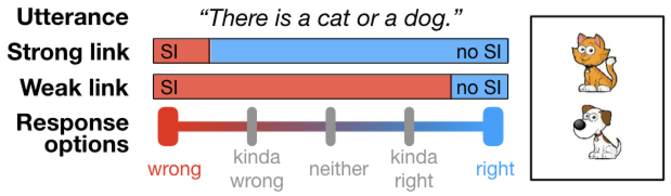
\includegraphics{writeup_files/figure-latex/linkvisualization-1} 

}

\caption{Strong and weak link from response options to researcher inference about scalar implicature rate, exemplified for the disjunctive utterance when the conjunction is true.}\label{fig:linkvisualization}
\end{figure}

Let's examine an example. Assume three response options (wrong, neither,
right). Assume further that a third of participants each gave each of
the three responses, i.e., the distributions of responses is 1/3, 1/3,
and 1/3. Under the Strong link, we infer that this task yielded an
implicature rate of 2/3. Under the Weak link, we infer that this task
yielded an implicature rate of 1/3. This is quite a drastic difference
if we are for instance interested in whether scalar implicatures are
inference defaults and we would like to interpret an implicature rate of
above an arbitrary threshold (e.g., 50\%) as evidence for such a claim.
Under the Strong link, we would conclude that scalar implicatures are
not defaults. Under the Weak link, we would conclude that they are.

In the experiment reported in the following section, we presented
participants with exactly this setup. Different groups of participants
were presented with different numbers of response options. We
categorized their responses according to the Weak and the Strong link
and tested whether number of response options and categorization scheme
leads to different conclusions about implicature rates.

\section{Experiment}\label{experiment}

\subsection{Methods}\label{methods}

\subsubsection{Participants}\label{participants}

200 participants were recruited using Amazon Mechanical Turk (binary=50,
ternary53, quaternary=43, quinary=54). No participant was excluded from
the final analysis.

\subsubsection{Procedure}\label{procedure}

The study was administered online through Amazon Mechanical Turk.
Participants were introduced to a set of cards with pictures of one or
two animals (Figure \ref{fig:stimuli}). They were told that a
blindfolded fictional character called Bob is going to guess what
animals are on the card. On each trial, participants saw a card as well
as a sentence representing Bob's guess. For example, they saw a card
with a cat on it and read the sentence \enquote{There is a cat on the
card.} The study ended after 24 trials. At the end participants
optionally provided demographic information. You can access and view
\href{**XXX\%20masoud\%20insert\%20link**}{the online study here}.

\subsubsection{Design and Materials}\label{design-and-materials}

\begin{figure}[t]

{\centering 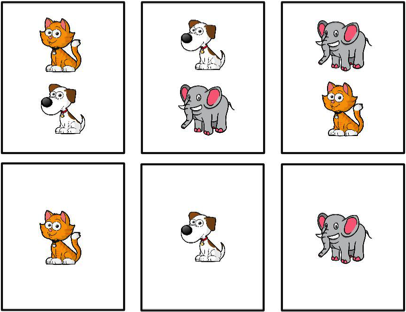
\includegraphics{writeup_files/figure-latex/stimuli-1} 

}

\caption{Cards used in the connective guessing game.}\label{fig:stimuli}
\end{figure}

The design had two main manipulaitons: the type of card and the type of
guess. There were two types of cards. Cards with only one animal on them
and cards with two animals. Animals were chosen from the following set:
cat, dog, and elephant There were three types of guesses: simple (e.g.
\emph{There is a cat}), conjunctive (e.g. \emph{There is a cat and a
dog}), and disjunctive (e.g. \emph{There is a cat or a dog}).

In each trial, the animal labels used in the guess and the animal images
on the card may have no overlap (e.g.~Image: dog, Guess: \emph{There is
a cat or an elephant}), a partial overlap (e.g.~Image: Cat, Guess:
\emph{There is a cat or an elephant}), or a total overlap (e.g.~Image:
cat and elephant, Guess: \emph{There is a cat or an elephant}). Crossing
the number of animals on the card, the type of guess, and the overlap
between the guess and the card results in 12 different possible trial
types. We chose 8 trial types (Figure \ref{fig:trials}), balancing the
number of one-animal vs.~two-animal cards, simple vs.~connective
guesses, and expected true vs.~false trials.

The study used five different types of measurements. 1. two-options
(true vs.~false) 2. two-options (wrong vs.~right) 3. three-options
(wrong, neither, right) 4. four-options (wrong, kinda wrong, kinda
right, right) 5. five-options (wrong, kinda wrong, neither, kinda right,
right).

\begin{figure}[t]

{\centering 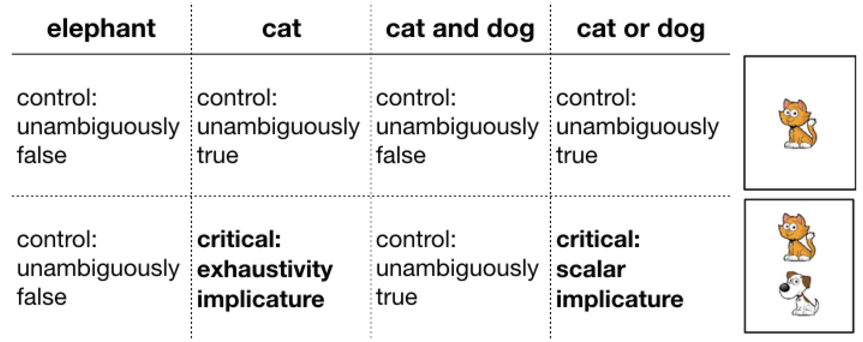
\includegraphics{writeup_files/figure-latex/trials-1} 

}

\caption{Trial types represented by example cards and guesses.}\label{fig:trials}
\end{figure}

\subsection{Results}\label{results}

We are primarily concerned with the \enquote{rate of implicatures} in an
experimental study. Two trial types are predicted to include pragmatic
implicatures. First, trials where there are two animals on the card but
the fictional character guesses using the connective \emph{or}; for
example \enquote{cat or dog} when the card has both a cat and a dog on
it. We call such trials \enquote{scalar} trials. Second, trials where
there are two animals on the card but the character guesses only one;
for example \enquote{cat} when the card has a cat and a dog on it. We
call such trials \enquote{exhaustive}. In our assessment of implicature
rate we focus on these two types of trials.

We define \enquote{implicature rate} in two ways:

This study set out to test two hypotheses. First, that the proportion of
pragmatic vs.~literal responses in a truth values judgement task changes
based on the number of response options available to the participants.
We test this hypothesis formally using a binomial mixed effects model
with the fixed effect of response type and the random intercept for
participants as well as random intercept and slope for

A second hypothesis was that the definition of what responses count as
participants computing an implicature may affect the estimated rate of
implicature in the experimental task.

\begin{figure}[t]

{\centering 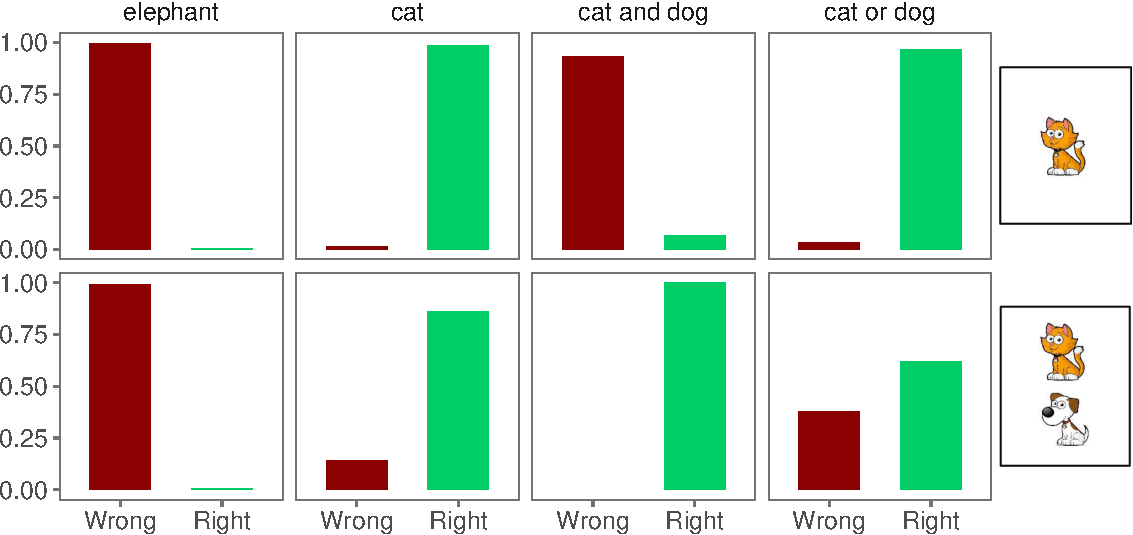
\includegraphics{writeup_files/figure-latex/binaryPlot-1} 

}

\caption{Adults' two-alternative forced choice judgments in the connective guessing game.}\label{fig:binaryPlot}
\end{figure}

\begin{figure}[t]

{\centering 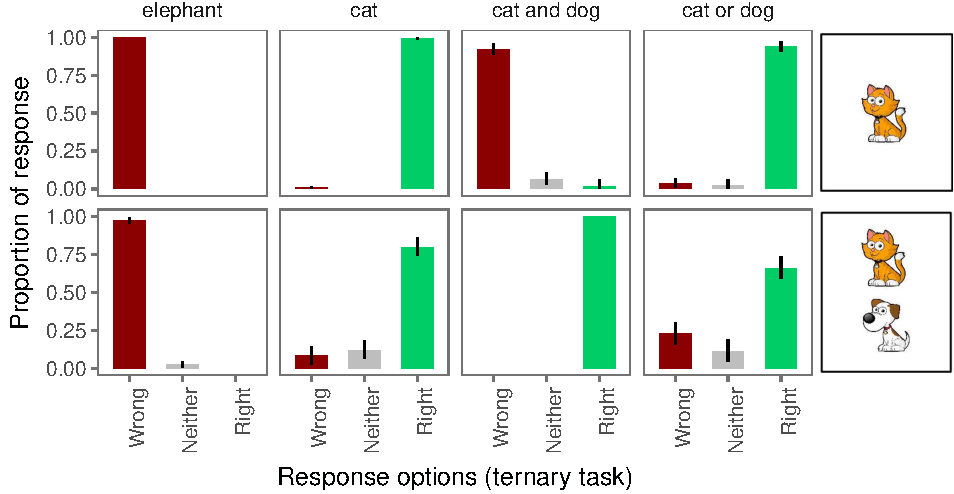
\includegraphics{writeup_files/figure-latex/ternaryPlot-1} 

}

\caption{Adults' three-alternative forced choice judgments in the connective guessing game.}\label{fig:ternaryPlot}
\end{figure}

\begin{figure}[t]

{\centering 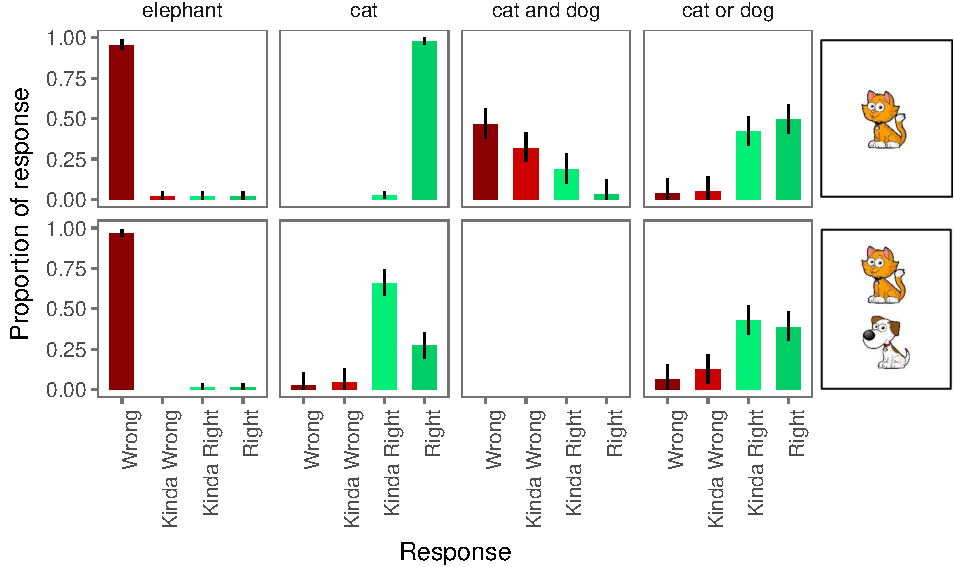
\includegraphics{writeup_files/figure-latex/quaternaryPlot-1} 

}

\caption{Adults' three-alternative forced choice judgments in the connective guessing game.}\label{fig:quaternaryPlot}
\end{figure}

\begin{figure}[t]

{\centering 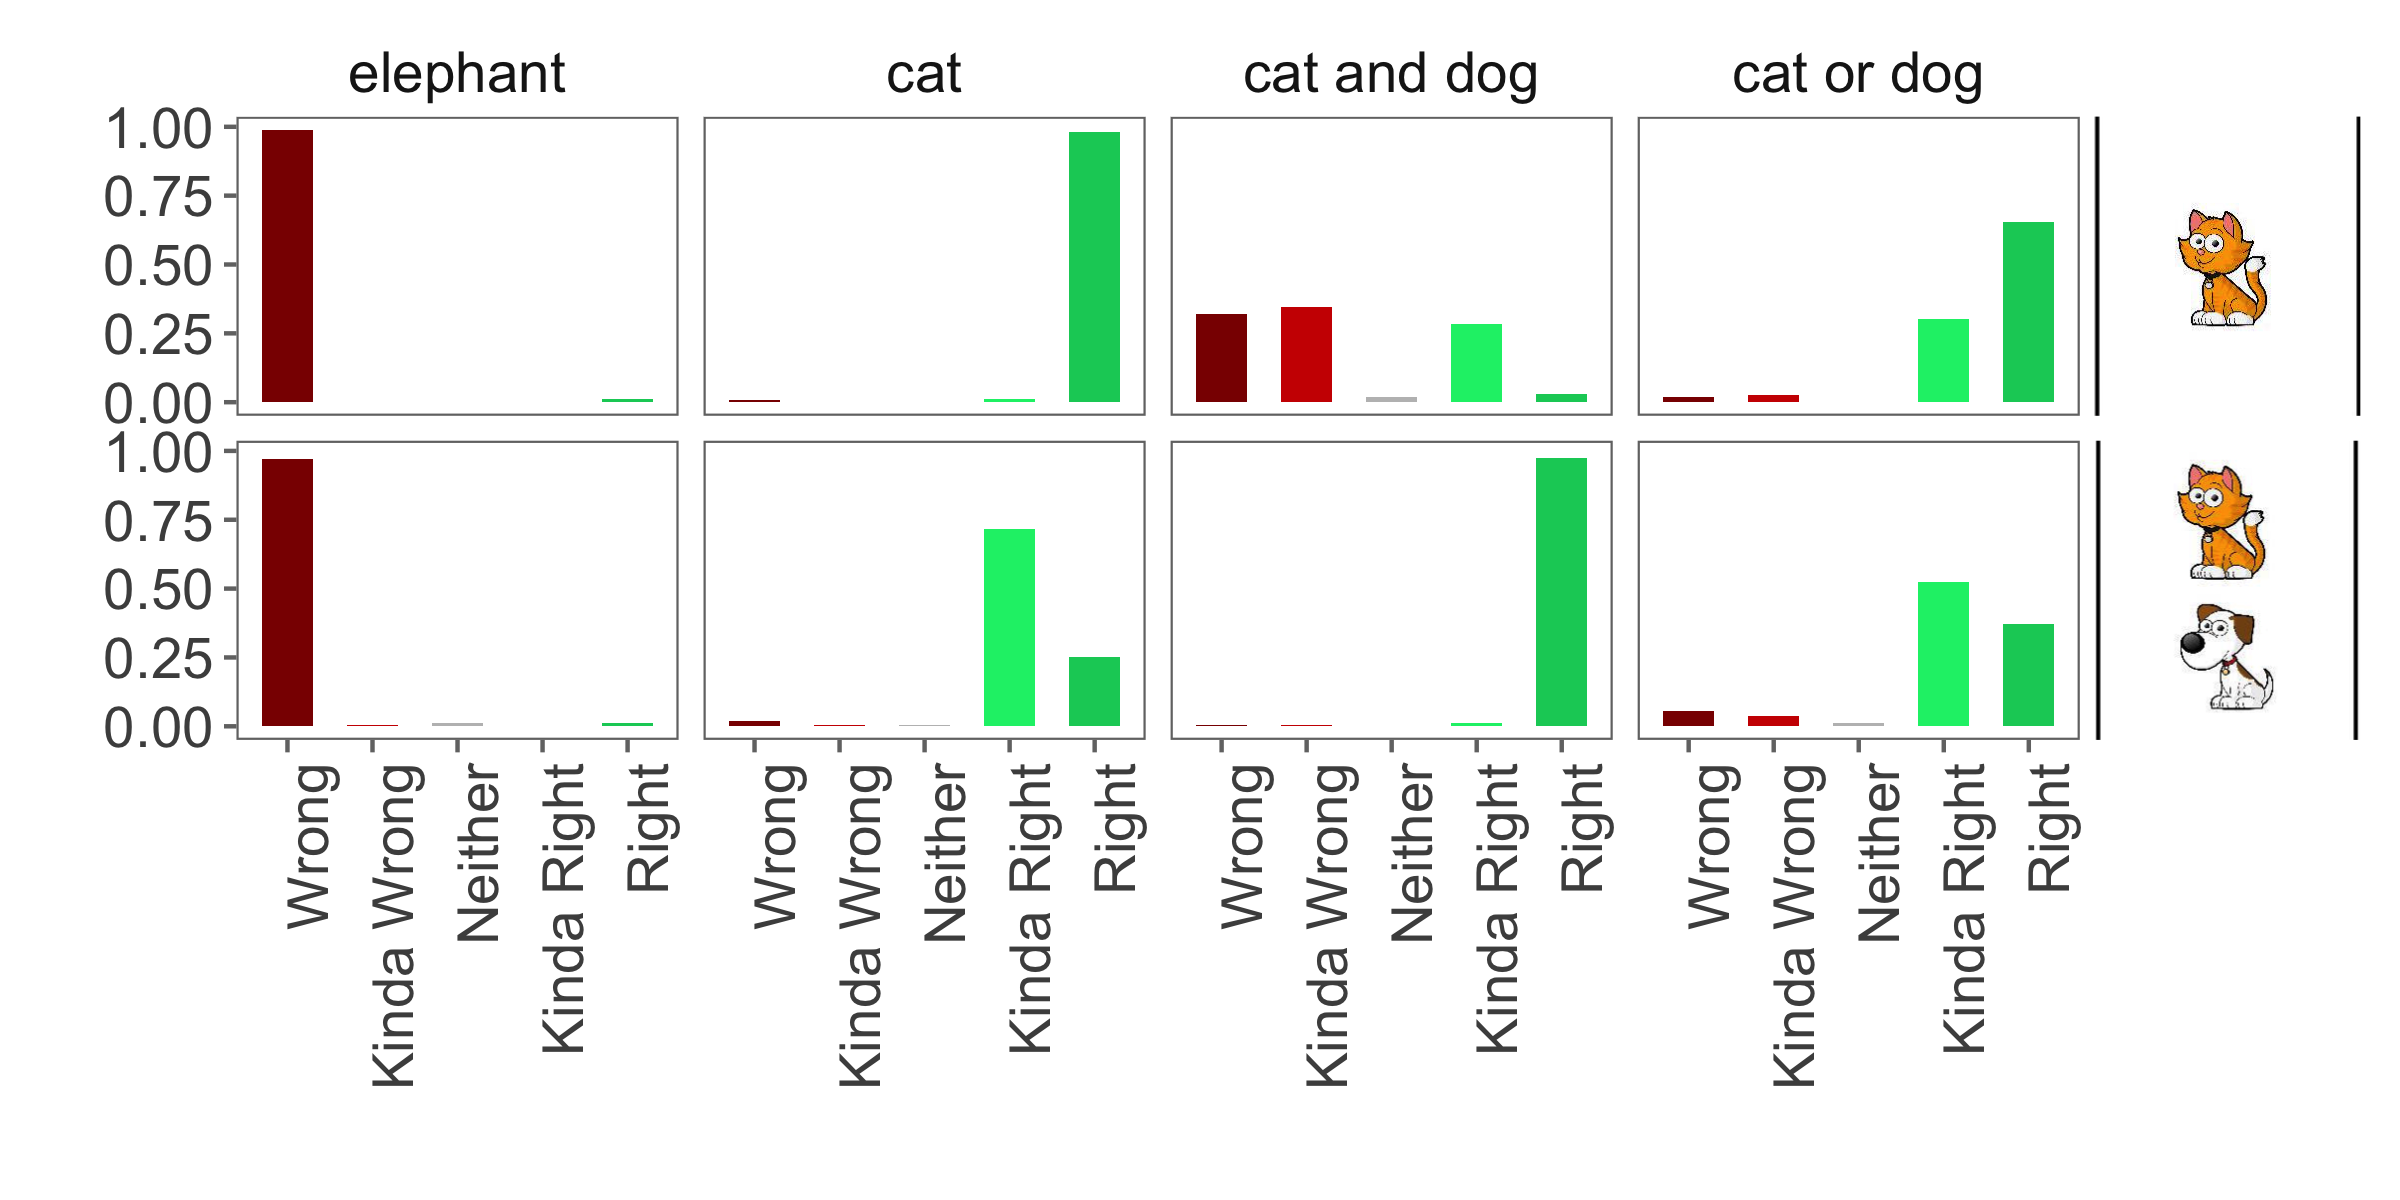
\includegraphics{writeup_files/figure-latex/quinaryPlot-1} 

}

\caption{Adults' three-alternative forced choice judgments in the connective guessing game.}\label{fig:quinaryPlot}
\end{figure}

\begin{figure}
\centering
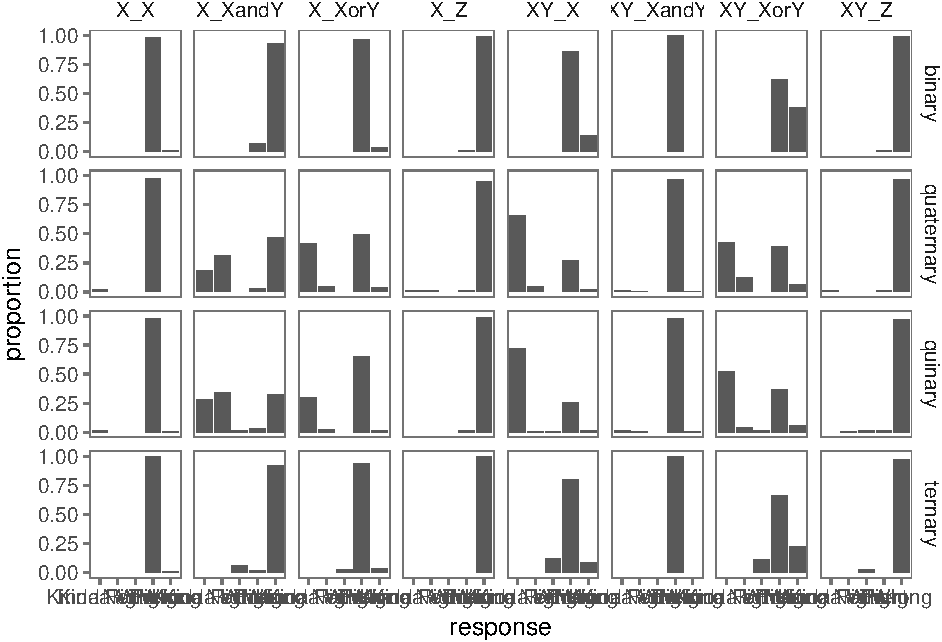
\includegraphics{writeup_files/figure-latex/unnamed-chunk-2-1.pdf}
\caption{}
\end{figure}

\begin{itemize}
\tightlist
\item
  make sure to break down based on whether participants had logical
  training or not.
\end{itemize}

\subsubsection{Analysis}\label{analysis}

\begin{figure}
\centering
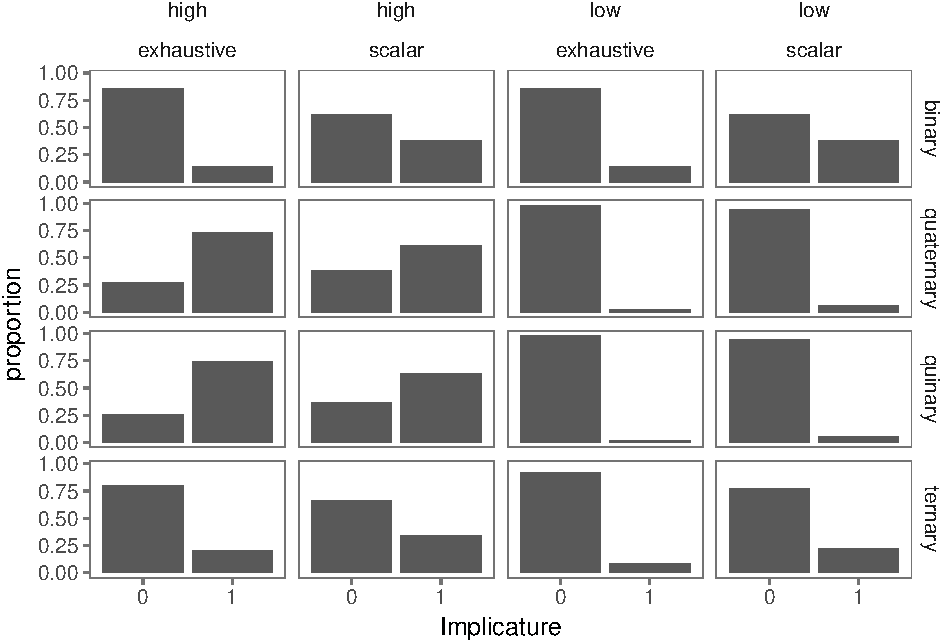
\includegraphics{writeup_files/figure-latex/unnamed-chunk-3-1.pdf}
\caption{}
\end{figure}

\begin{verbatim}
## Warning in (function (fn, par, lower = rep.int(-Inf, n), upper =
## rep.int(Inf, : failure to converge in 10000 evaluations
\end{verbatim}

\begin{verbatim}
## Warning in checkConv(attr(opt, "derivs"), opt$par, ctrl = control
## $checkConv, : Model failed to converge with max|grad| = 0.524298 (tol =
## 0.001, component 1)
\end{verbatim}

\begin{verbatim}
## Generalized linear mixed model fit by maximum likelihood (Laplace
##   Approximation) [glmerMod]
##  Family: binomial  ( logit )
## Formula: implicature ~ definition * response_type + trial_type + (1 +  
##     response_type | card) + (1 | participant)
##    Data: implicature_rate
## 
##      AIC      BIC   logLik deviance df.resid 
##   1783.4   1899.0   -871.7   1743.4     2380 
## 
## Scaled residuals: 
##     Min      1Q  Median      3Q     Max 
## -7.8815 -0.2261 -0.1198  0.2334 10.0887 
## 
## Random effects:
##  Groups      Name                    Variance Std.Dev. Corr             
##  participant (Intercept)             5.224316 2.28568                   
##  card        (Intercept)             0.008402 0.09166                   
##              response_typequaternary 0.084138 0.29007  -1.00            
##              response_typequinary    0.003720 0.06099  -0.79  0.81      
##              response_typeternary    0.044946 0.21201   0.90 -0.89 -0.67
## Number of obs: 2400, groups:  participant, 200; card, 3
## 
## Fixed effects:
##                                       Estimate Std. Error z value Pr(>|z|)
## (Intercept)                           -2.64555    0.43138  -6.133 8.63e-10
## definitionlow                         -0.02508    0.24943  -0.101    0.920
## response_typequaternary                3.47868    0.61328   5.672 1.41e-08
## response_typequinary                   3.44163    0.55426   6.209 5.32e-10
## response_typeternary                   0.29732    0.56967   0.522    0.602
## trial_typescalar                       0.85657    0.13861   6.180 6.41e-10
## definitionlow:response_typequaternary -6.08294    0.61009  -9.970  < 2e-16
## definitionlow:response_typequinary    -5.71913    0.50693 -11.282  < 2e-16
## definitionlow:response_typeternary    -1.21490    0.36931  -3.290    0.001
##                                          
## (Intercept)                           ***
## definitionlow                            
## response_typequaternary               ***
## response_typequinary                  ***
## response_typeternary                     
## trial_typescalar                      ***
## definitionlow:response_typequaternary ***
## definitionlow:response_typequinary    ***
## definitionlow:response_typeternary    ** 
## ---
## Signif. codes:  0 '***' 0.001 '**' 0.01 '*' 0.05 '.' 0.1 ' ' 1
## 
## Correlation of Fixed Effects:
##                     (Intr) dfntnl rspns_typqt rspns_typqn rspns_typt
## definitinlw         -0.287                                          
## rspns_typqt         -0.724  0.202                                   
## rspns_typqn         -0.760  0.224  0.554                            
## rspns_typtr         -0.643  0.218  0.418       0.510                
## trl_typsclr         -0.218 -0.001  0.060       0.065       0.007    
## dfntnlw:rspns_typqt  0.214 -0.408 -0.330      -0.167      -0.101    
## dfntnlw:rspns_typqn  0.217 -0.492 -0.156      -0.309      -0.116    
## dfntnlw:rspns_typt   0.220 -0.675 -0.155      -0.170      -0.280    
##                     trl_ty dfntnlw:rspns_typqt dfntnlw:rspns_typqn
## definitinlw                                                       
## rspns_typqt                                                       
## rspns_typqn                                                       
## rspns_typtr                                                       
## trl_typsclr                                                       
## dfntnlw:rspns_typqt -0.098                                        
## dfntnlw:rspns_typqn -0.103  0.266                                 
## dfntnlw:rspns_typt  -0.036  0.298               0.349             
## convergence code: 0
## Model failed to converge with max|grad| = 0.524298 (tol = 0.001, component 1)
## failure to converge in 10000 evaluations
\end{verbatim}

\section{Discussion}\label{discussion}

Alternative Linking Hypothesis: * RSA: Response behavior across
conditions (utterance-card combinations) and dependent measures can be
predicted by a linking hypothesis that assumes that participants are
behaving like soft-optimal RSA speakers and provide a particular
response (eg TRUE) to an utterance u if the RSA speaker probability of u
(given the card) is within a particular probability interval (eg, within
the interval {[}theta, 1{]}).

\begin{itemize}
\tightlist
\item
  Differences between traditional approaches and RSA: 1. The traditional
  linking hypotheses are based on a binary implicature/literal theory of
  pragmatic reasoning but RSA gives a continuous measure of pragmatic
  reasoning and allows for better predicting response behavior with
  multiple options.
\end{itemize}

\newpage

\section{References}\label{references}

\setlength{\parindent}{-0.5in} \setlength{\leftskip}{0.5in}

\hypertarget{refs}{}
\hypertarget{ref-Barner2011}{}
Barner, D., Brooks, N., \& Bale, A. (2011). Accessing the unsaid: the
role of scalar alternatives in children's pragmatic inference.
\emph{Cognition}, \emph{118}(1), 84--93.
doi:\href{https://doi.org/10.1016/j.cognition.2010.10.010}{10.1016/j.cognition.2010.10.010}

\hypertarget{ref-Bergen2012}{}
Bergen, L., \& Grodner, D. J. (2012). Speaker knowledge influences the
comprehension of pragmatic inferences. \emph{Journal of Experimental
Psychology. Learning, Memory, and Cognition}, \emph{38}(5), 1450--60.
doi:\href{https://doi.org/10.1037/a0027850}{10.1037/a0027850}

\hypertarget{ref-Bonnefon2009}{}
Bonnefon, J.-F., Feeney, A., \& Villejoubert, G. (2009). When some is
actually all: scalar inferences in face-threatening contexts.
\emph{Cognition}, \emph{112}(2), 249--58.
doi:\href{https://doi.org/10.1016/j.cognition.2009.05.005}{10.1016/j.cognition.2009.05.005}

\hypertarget{ref-Bott2004}{}
Bott, L., \& Noveck, I. (2004). Some utterances are underinformative:
The onset and time course of scalar inferences. \emph{Journal of Memory
and Language}, \emph{51}(3), 437--457.
doi:\href{https://doi.org/10.1016/j.jml.2004.05.006}{10.1016/j.jml.2004.05.006}

\hypertarget{ref-Breheny2013}{}
Breheny, R., Ferguson, H. J., \& Katsos, N. (2013). Taking the epistemic
step: Toward a model of on-line access to conversational implicatures.
\emph{Cognition}, \emph{126}(3), 423--40.
doi:\href{https://doi.org/10.1016/j.cognition.2012.11.012}{10.1016/j.cognition.2012.11.012}

\hypertarget{ref-Breheny2006}{}
Breheny, R., Katsos, N., \& Williams, J. (2006). Are generalised scalar
implicatures generated by default? An on-line investigation into the
role of context in generating pragmatic inferences. \emph{Cognition},
\emph{100}(3), 434--63.
doi:\href{https://doi.org/10.1016/j.cognition.2005.07.003}{10.1016/j.cognition.2005.07.003}

\hypertarget{ref-Chemla2011}{}
Chemla, E., \& Spector, B. (2011). Experimental Evidence for Embedded
Scalar Implicatures. \emph{Journal of Semantics}, \emph{28}(3),
359--400.

\hypertarget{ref-DeNeys2007}{}
De Neys, W., \& Schaeken, W. (2007). When People Are More Logical Under
Cognitive Load - Dual Task Impact on Scalar Implicature.
\emph{Experimental Psychology}, \emph{54}(2), 128--133.
doi:\href{https://doi.org/10.1027/1618-3169.54.2.128}{10.1027/1618-3169.54.2.128}

\hypertarget{ref-Degen2015}{}
Degen, J. (2015). Investigating the distribution of 'some' (but not
'all') implicatures using corpora and web-based methods. \emph{Semantics
and Pragmatics}, \emph{8}(11), 1--55.
doi:\href{https://doi.org/10.3765/sp.8.11}{10.3765/sp.8.11}

\hypertarget{ref-Degen2014}{}
Degen, J., \& Goodman, N. D. (2014). Lost your marbles? The puzzle of
dependent measures in experimental pragmatics. \emph{Proceedings of the
36th Annual Conference of the Cognitive Science Society}, 397--402.

\hypertarget{ref-DegenTanenhaus2015}{}
Degen, J., \& Tanenhaus, M. K. (2015). Processing scalar implicature A
constraint-based approach. \emph{Cognitive Science}, \emph{39}(4),
667--710.
doi:\href{https://doi.org/10.1111/cogs.12171}{10.1111/cogs.12171}

\hypertarget{ref-DegenTanenhaus2016}{}
Degen, J., \& Tanenhaus, M. K. (2016). Availability of Alternatives and
the Processing of Scalar Implicatures: A Visual World Eye-Tracking
Study. \emph{Cognitive Science}, \emph{40}(1), 172--201.
doi:\href{https://doi.org/10.1111/cogs.12227}{10.1111/cogs.12227}

\hypertarget{ref-Doran2012}{}
Doran, R., Ward, G., Larson, M., McNabb, Y., \& Baker, R. E. (2012). A
novel experimental paradigm for distinguishing between what is said and
what is implicated. \emph{Language}, \emph{88}, 124--154.

\hypertarget{ref-Geurts2009}{}
Geurts, B., \& Pouscoulous, N. (2009). Embedded implicatures?!?
\emph{Semantics and Pragmatics}, \emph{2}, 1--34.
doi:\href{https://doi.org/10.3765/sp.2.4}{10.3765/sp.2.4}

\hypertarget{ref-grice1975}{}
Grice, H. P. (1975). Logic and Conversation. \emph{Syntax and
Semantics}, \emph{3}, 41--58. Retrieved from
\href{http://books.google.com/books?hl=en\%7B/\&\%7Dlr=\%7B/\&\%7Did=hQCzOmaGeVYC\%7B/\&\%7Doi=fnd\%7B/\&\%7Dpg=PA121\%7B/\&\%7Ddq=Logic+and+conversation\%7B/\&\%7Dots=j7aijUymwm\%7B/\&\%7Dsig=iV1rz1eEm4ns6bQ6CevIURXFVO4}{http://books.google.com/books?hl=en\{\textbackslash{}\&\}lr=\{\textbackslash{}\&\}id=hQCzOmaGeVYC\{\textbackslash{}\&\}oi=fnd\{\textbackslash{}\&\}pg=PA121\{\textbackslash{}\&\}dq=Logic+and+conversation\{\textbackslash{}\&\}ots=j7aijUymwm\{\textbackslash{}\&\}sig=iV1rz1eEm4ns6bQ6CevIURXFVO4}

\hypertarget{ref-Grodner2010}{}
Grodner, D. J., Klein, N. M., Carbary, K. M., \& Tanenhaus, M. K.
(2010). ``Some,'' and possibly all, scalar inferences are not delayed:
Evidence for immediate pragmatic enrichment. \emph{Cognition},
\emph{116}(1), 42--55.
doi:\href{https://doi.org/10.1016/j.cognition.2010.03.014}{10.1016/j.cognition.2010.03.014}

\hypertarget{ref-horn1984}{}
Horn, L. (1984). Toward a new taxonomy for pragmatic inference: Q-based
and R-based implicature. In D. Schiffrin (Ed.), \emph{Meaning, form, and
use in context: Linguistic applications} (pp. 11--42). Washington:
Georgetown University Press.

\hypertarget{ref-huang2009}{}
Huang, Y. T., \& Snedeker, J. (2009). On-line interpretationf of scalar
quantifiers: Insight into the semantics-pragmatics interface.
\emph{Cognitive Psychology}, \emph{58}, 376--415.

\hypertarget{ref-Katsos2011}{}
Katsos, N., \& Bishop, D. V. M. (2011). Pragmatic tolerance:
implications for the acquisition of informativeness and implicature.
\emph{Cognition}, \emph{120}(1), 67--81.
doi:\href{https://doi.org/10.1016/j.cognition.2011.02.015}{10.1016/j.cognition.2011.02.015}

\hypertarget{ref-levinson2000}{}
Levinson, S. C. (2000). \emph{Presumptive Meanings - The Theory of
Generalized Conversational Implicature}. MIT Press.

\hypertarget{ref-DeMarneffe2017}{}
Marneffe, M.-C. de, \& Tonhauser, J. (2016). Inferring meaning from
indirect answers to polar questions: The contribution of the
rise-fall-rise contour. In E. Onea, M. Zimmermann, \& K. von Heusinger
(Eds.), \emph{Questions in discourse}. Leiden: Brill Publishing.

\hypertarget{ref-Musolino2004}{}
Musolino, J. (2004). The semantics and acquisition of number words:
integrating linguistic and developmental perspectives. \emph{Cognition},
\emph{93}(1), 1--41.
doi:\href{https://doi.org/10.1016/j.cognition.2003.10.002}{10.1016/j.cognition.2003.10.002}

\hypertarget{ref-Noveck2001}{}
Noveck, I. (2001). When children are more logical than adults:
experimental investigations of scalar implicature. \emph{Cognition},
\emph{78}(2), 165--188. Retrieved from
\url{http://www.ncbi.nlm.nih.gov/pubmed/11074249}

\hypertarget{ref-noveck2008}{}
Noveck, I. A., \& Reboul, A. (2008). Experimental pragmatics: a Gricean
turn in the study of language. \emph{Trends in Cognitive Sciences},
\emph{12}(11), 425--431.
doi:\href{https://doi.org/10.1016/j.tics.2008.07.009}{10.1016/j.tics.2008.07.009}

\hypertarget{ref-Noveck2003}{}
Noveck, I., \& Posada, A. (2003). Characterizing the Time Course of an
Implicature: an Evoked Potentials Study. \emph{Brain and Language},
\emph{85}(2), 203--210.
doi:\href{https://doi.org/10.1016/S0093-934X(03)00053-1}{10.1016/S0093-934X(03)00053-1}

\hypertarget{ref-Papafragou2004}{}
Papafragou, A., \& Tantalou, N. (2004). Children's Computation of
Implicatures. \emph{Language Acquisition}, \emph{12}(1), 71--82.

\hypertarget{ref-Politzer-Ahles2013}{}
Politzer-Ahles, S., \& Fiorentino, R. (2013). The Realization of Scalar
Inferences: Context Sensitivity without Processing Cost. \emph{PLoS
ONE}, \emph{8}(5).
doi:\href{https://doi.org/10.1371/journal.pone.0063943}{10.1371/journal.pone.0063943}

\hypertarget{ref-VanTiel2014}{}
Tiel, B. van, Miltenburg, E. van, Zevakhina, N., \& Geurts, B. (2014).
Scalar diversity. \emph{Journal of Semantics}.
doi:\href{https://doi.org/10.1093/jos/ffu017}{10.1093/jos/ffu017}

\hypertarget{ref-Zondervan2010}{}
Zondervan, A. (2010). \emph{Scalar implicatures or focus: an
experimental approach} (PhD thesis). Universiteit Utrecht, Amsterdam.






\end{document}
